%************************************************
\section{Automatic Subscription Handling}\label{ch:automaticsubscription}
%************************************************

After defining the notation and functionality provided to the user through the BPMN extension for flexible event subscription, this chapter describes the changes necessary to the software infrastructure to implement the execution semantics.
The concept requires that all subscription operations and event handling is executed by the system itself, solely based on the extended BPMN model.
Changes are necessary to both, the event processing module and the process engine. This chapter attempts to keep the change descriptions general so they can be applied to any common process engine and event processing platform.
The first section describes the necessary extension to the event processing so that a delayed delivery of events is supported.
The following \autoref{ch:extendedprocessengine} specifies the changes necessary to the behavior of the process engine as the connecting element between the BPMN model and the event processing platform.


\subsection{Buffered Event Processing}\label{ch:bufferedcep}
When reduced to the basics, a standard event processing platform works as follows: The user subscribes to events providing an event query and a notification-path. The platform responds with a unique identifier for that subscription.
Whenever an event occurs that matches the provided query, the platform issues a notification to the notification-path. Subscriptions can be deleted through their unique identifier.
These two operations, \textit{subscribe} and \textit{unsubscribe}, make the fundamental \acs{API} of a CEP platform~(see \autoref{ch:bg:cep}).

\paragraph{An API for buffered event processing}
The novel BPMN extension for flexible event subscription allows to issue a subscription to an event source well before the events ought to be delivered to the process instance. The introduction of an event buffer as a separate entity between the notification-recipients and the event query makes an adaptation of the API necessary.
In the following, we propose an API for buffered event processing which provides the functionality necessary to implement the execution semantics specified in the BPMN extension. Note that the proposal is not restricted to a certain kind of technology or protocol to implement the API.

Firstly, the \textit{subscribe} operation has to be available in two steps:

\begin{aenumerate}
	\item \textit{registerQuery(queryString[, bufferPolicies]): queryId}\newline
	The call registers an event query in the CEP platform and instantiates a buffer. Matching events will be held in the buffer according to the specified  policies. It returns a unique identifier to that new query registration and hence for the connected buffer. That identifier must be used to modify the query later.
	
	\textit{bufferPolicies} is an optional parameter which is provided as an object with four possible fields: \textit{LifetimePolicy}, \textit{ConsumptionPolicy}, \textit{SizePolicy}, \textit{OrderPolicy}. Refer to \autoref{ch:bpmnx:bufferpolicies} for a detailed specification of the semantics and possible values of the parameters. If \textit{bufferPolicies} is not or only partly specified, the system should fall back to the denoted default values.
	
	\item \textit{subscribe(queryId, notificationPath): subscriptionId}\newline
	Initiates the delivery of notifications for a given queryId to a notification recipient.
	The recipient is specified through the \textit{notificationPath}, the full address of the entity that is supposed to receive the message.
	Notifications are delivered asynchronously as soon as they are available. If the buffer is not empty, a message will be sent right after the \textit{requestEvents} call.
	A similar operation, \textit{addNotificationRecipient}, is available in existing CEP platforms. It adds a notification recipient to a query that is already registered in the platform. The difference is in the delivery of the first buffered message: \textit{requestEvents} sends out the message from the buffer, \textit{addNotificationRecipient} will send out notifications only for future query output.
\end{aenumerate}\label{def:apiextension-subscribe}

\noindent A similar situation holds for the un-subscribe operation: Given flexible event subscription, the operation must comprise of two steps:

\begin{aenumerate}
	\setcounter{enumi}{2}
	\item \textit{unsubscribe(subscriptionId)}\newline
	Removes a notification-recipient for a given query-id. Note that the buffer and query instance remain intact, so that other recipients can still subscribe.
	\item \textit{removeQuery(queryId)}\newline
	Completely deletes the query and its buffer, so that no notifications are sent out any longer. 
\end{aenumerate}\label{def:apiextension-unsubscribe}

\noindent
All four methods must be available to execute a subscription before process deployment.
The query must be registered using \textit{registerQuery} before the process instance, and hence the notification-path, is available. For each process instance, a subscription can be issued individually using \textit{subscribe} and thereafter, the notification-recipient can be removed with \textit{unsubscribe}.
The query and its buffer will remain active even after any single instance has terminated. When the process gets un-deployed, the query can be deleted using \textit{removeQuery}.
%\autoref{ch:extendedprocessengine} describes the steps in detail.


\paragraph{Architectural options}

Three options are considered to implement the explained functionality~(\autoref{fig:buffered-event-handling-architecture}). 
(a) It can either be implemented by adopting the CEP platform itself, (b) by implementing a separate middleware between process engine and CEP platform, (c) or by implementing a buffering module as part of the process engine.
Which of the three options suits best has to be evaluated for the given use-case and existing infrastructure. In some cases it might not be possible to adapt the code of process engine or event processing platform, which leaves a separate middleware as the only choice.

A reference implementation for an extended complex event processing platform is presented in \autoref{ch:implunicorn} at the example of the Esper-based CEP~platform \textit{Unicorn}. It also explains, why extending the event platform was the preferred choice in the given scenario.

\begin{figure}[]
	\myfloatalign
	{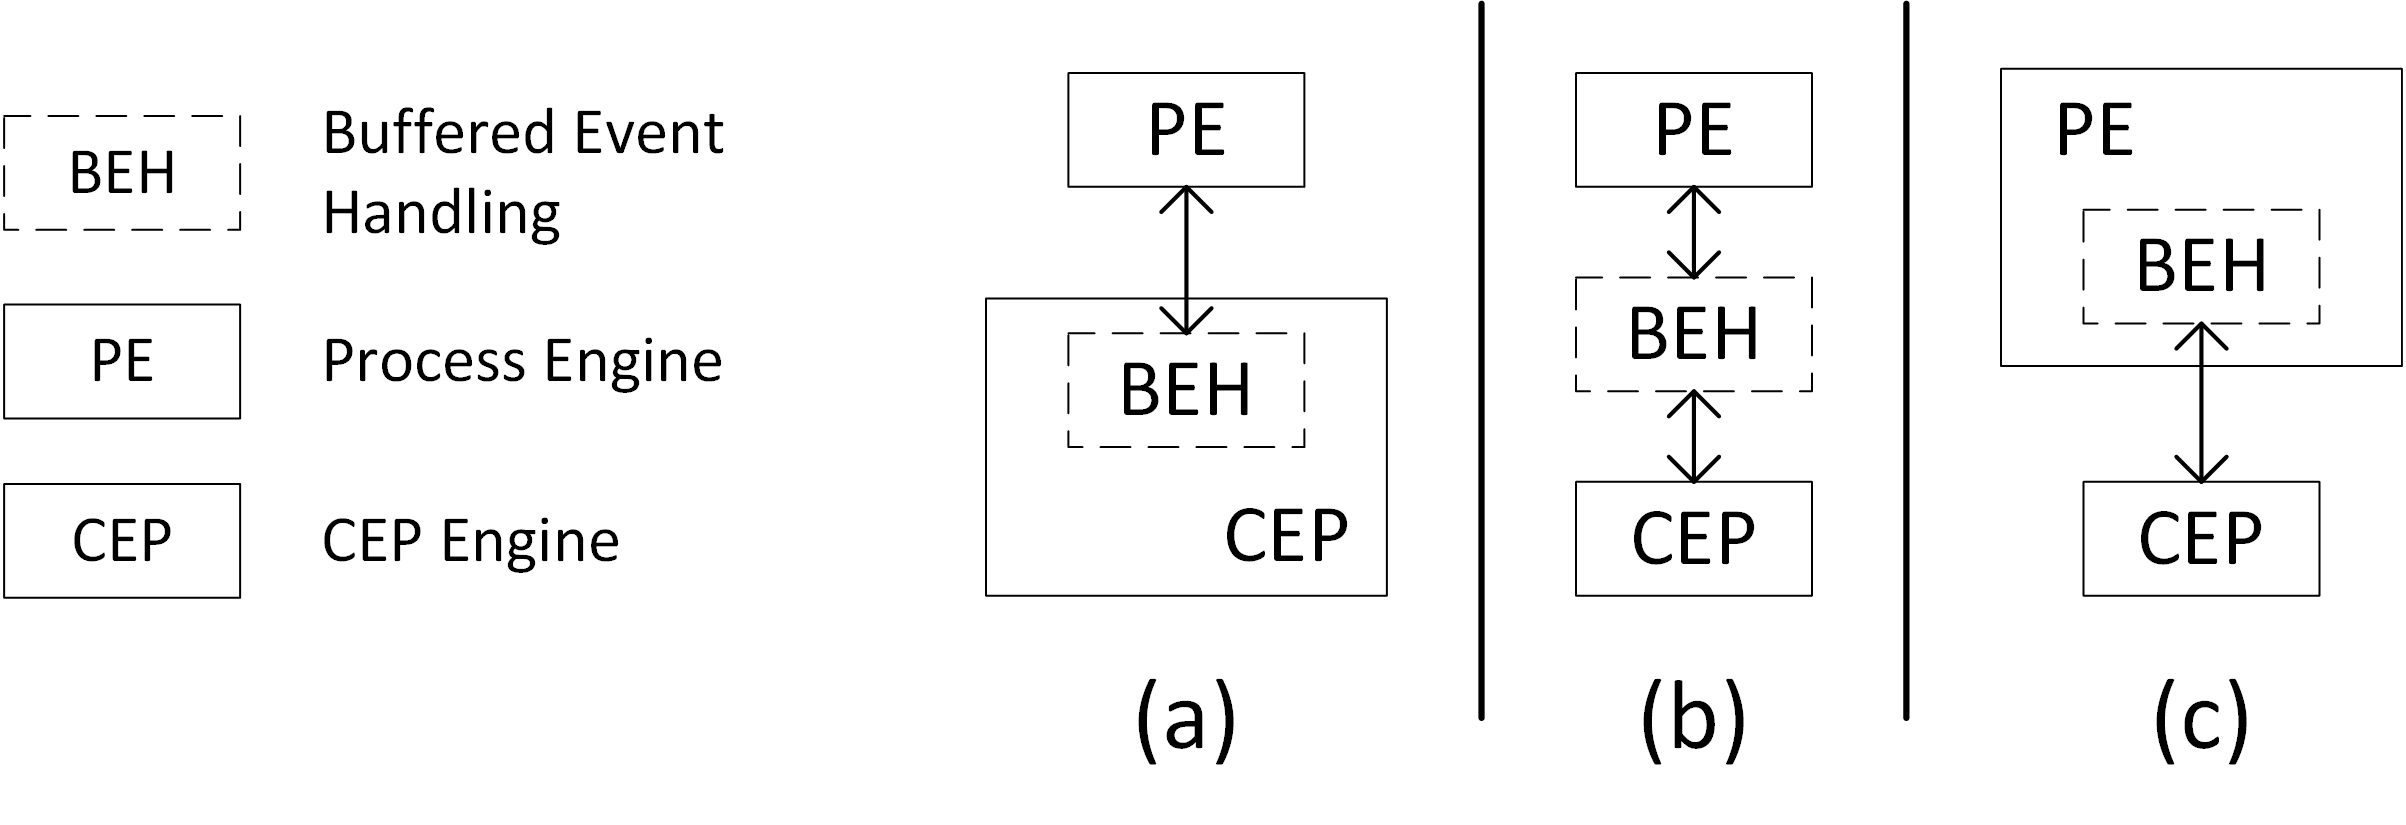
\includegraphics[width=0.8\linewidth]{chapters/concept/automaticsubscription/architecture-options.png}}
	\caption{Architectural options to implement the event buffers}
	\label{fig:buffered-event-handling-architecture}
\end{figure}


\subsection{Extended Process Engine Behavior}\label{ch:extendedprocessengine}
It is the task of the Business Process Engine to interpret and execute process models and connect to an event processing platform in event-driven setups.
From the three relevant parts, two have already been defined, the BPMN extension and the buffered event processing module.
Out of the box, a process engine like Camunda will ignore any proprietary BPMN extensions and the subscription to an event source must be especially implemented. An example for such an implementation is provided in \autoref{ass:model:buffered}.
One goal of this work is to automatize the handling of event subscriptions solely based on the information available through the extended BPMN model. Additional process elements should not be required.
This section will clarify, which operations need to be executed by the process engine to enable the automatic subscription handling.
\autoref{ch:implcamunda} demonstrates the implementation of automatic subscription handling at the example of Camunda.

\paragraph{Parsing additional information from the BPMN model}
It is required that the process engine is able to read the additional information from the BPMN extension~(see~\autoref{ch:bpmnx}) so that it is available during process deployment and execution.
This affects the BPMN message element, which can contain the additional attributes \textit{eventQuery}, \textit{subscriptionTime} and \textit{bufferPolicies}.
Secondly, the \textit{Event Subscription Task} has to be processed. It contains a reference to a Message entity within the same model element.
The process engine might have to be adopted to read all relevant data from the extended model.


\paragraph{Managing subscription and un-subscription}
As defined in the BPMN extension for flexible event subscription, the action of subscribing to an event source can happen at different times during process deployment and execution. The options and the implicit timing of subscription and un-subscription are specified in \autoref{ch:bpmnx:subscriptiontimes}.
The process engine must communicate with the process engine using the four calls \textit{registerQuery}, \textit{requestEvents}, \textit{unsubscribe} and \textit{deleteQuery}, that were presented in the previous chapter.
For each possible subscription time, the following briefly enumerates which operations must be executed when. 

\begin{description}
	\item[In every case:] 
		The return-value of \textit{registerQuery}, a unique identifier of that query, must be stored for the related BPMN \textit{Message}. The id is later necessary to execute the other three API methods.
		If the event query contains one or more variable values (see \autoref{ch:bpmnx:variables-in-queries}), all have to be replaced by their current values when \textit{registerQuery} is performed.
		When an event element is reached, a call to \textit{requestEvents} must be issued. When the execution of that event element is finished, call \textit{unsubscribe}.
	\item[Subscr. on process deployment:]
		When a process gets deployed, the process engine must check if subscription information is in the model. For every \textit{Message} element that is set as \textit{subscribe on pr. deployment}, a call to \textit{registerQuery} must be issued as part of the deployment process. A call to \textit{deleteQuery} is executed when the process gets un-deployed for the same messages.
	\item[Subscr. on process instantiation:] 
		When a process gets instantiated, \textit{registerQuery} must be executed for each \textit{Message} that is set to \textit{subscribe on pr. instantiation}. \textit{deleteQuery} can be called when the last reachable event element for a \textit{Message} has finished executing or no connected event can be reached anymore. The deletion happens at the latest when the process instance terminates.
	\item[Subscr. through explicit subscription task:]
		If the control flow reaches a subscription task, the process engine executes \textit{registerQuery} for the referenced \textit{Message}. The execution of \textit{deleteQuery} follows the same rules as in the preceding case.
	\item[Subscr. when the event element is reached:]
		Once the event element is reached, \textit{registerQuery} must be executed for any \textit{Message} that is not covered by one of the prior cases. \textit{deleteQuery} must be called when the event element is finished.
\end{description}
\todo[inline]{be more precise about the time the calls should be executed (if possible). "reached"? "completed"? use the right bpmn words}



\todo[inline]{write conclusions that repeat how each requirement has been fulfilled}
